\section{Results}\label{sec:results}

\subsection{Completion}
Table~\ref{tab:completion} shows how many of the \NEntries{} entries ended with a scored model. MICA built \NModelMica{} (\CompListMica\,\%), ModelAngelo \NModelAngelo{} (\CompListAngelo\,\%), EModelX(+AF) \NModelEmodelx{} (\CompListEmodelx\,\%), EMProt \NModelEmprot{} (\CompListEmprot\,\%), E3-CryoFold \NModelEthree{} (\CompListEthree\,\%), CryoAtom \NModelCryoatom{} (\CompListCryoatom\,\%) and CryoZeta \NModelCryozeta{} (\CompListCryozeta\,\%; \CompAttCryozeta\,\% of the \NRanCryozeta{} entries on which it was run). No run produced a file that could not be scored. The 9VI4 entry (1.8~\AA{}, a 1~GB map) failed for the five methods of the first version, and 26DK for MICA, EModelX(+AF) and E3-CryoFold; CryoAtom built a model for both (its run on 9VI4 took \RtMaxCryoatom{}~min), but ran out of GPU memory on \NFailedCryoatom{} other entries, \FailCrashListCryoatom{} (Table~\ref{tab:failures}, Appendix). CryoZeta did not run on every entry (Section~\ref{sec:added}). It failed on \NFailedCryozeta{}: 26DK and 9OC0 (killed by the system in the detection step of the program, also when they ran alone), 9Z24 (out of GPU memory at the chunk sizes 256 and 64, the second after 5.3~hours, then the 6-hour limit in the third attempt), 13BD (out of GPU memory in all four attempts) and, at the 6-hour limit, 9VBD and 9VUH (9VUH was run a second time, alone, and reached the limit again). It was not run on \NNotRunCryozeta{} entries (\NotRunListCryozeta{}): the system killed the run on 9VI4 while the other GPU was busy and there was no time left to run it again alone, and 9WFL and 9WME were cut by the end of a session twice (9WME three times), after 4.1 to 4.9~hours, because the free GPU time was used up. These are not failures of the method; they are left out of the comparisons and marked N in the tables. The three failures of MICA are limits of the free machine and not errors of the program: two kills by the system when MICA's model building used up the RAM, and one run that hit the 2-hour limit close to the end of its model building (the last gap of the last chain). They count as failures all the same, because the user who runs MICA on this machine does not get a model. Of the \NModelMica{} models, \NRerunMica{} (\RerunMicaList{}) needed a second attempt after a GPU out-of-memory failure of the first one (Section~\ref{sec:dockprocedure}).

\begin{table}[t]
\centering\small
\caption{Completion. \emph{Model scored}: the run ended with a model file that was scored. \emph{Failed}: crash, kill by the system or timeout. The last two columns divide by the 20 entries and by the entries on which the method was run (all 20).}
\label{tab:completion}
\fitwidth{\begin{tabular}{lrrrrrrr}
\toprule
Method & Entries & Model scored & Failed & No usable model & Not run & Completion, of 20 (\%) & of attempted (\%) \\
\midrule
MICA & 20 & 17 & 3 & 0 & 0 & 85 & 85 \\
ModelAngelo & 20 & 19 & 1 & 0 & 0 & 95 & 95 \\
EModelX(+AF) & 20 & 18 & 2 & 0 & 0 & 90 & 90 \\
EMProt & 20 & 19 & 1 & 0 & 0 & 95 & 95 \\
E3-CryoFold & 20 & 15 & 5 & 0 & 0 & 75 & 75 \\
CryoAtom & 20 & 16 & 4 & 0 & 0 & 80 & 80 \\
CryoZeta & 20 & 11 & 6 & 0 & 3 & 55 & 65 \\
\bottomrule
\end{tabular}
}
\end{table}

\subsection{Accuracy of the models that were built}
Table~\ref{tab:summary} and Figure~\ref{fig:heat} show the accuracy of each method on its own set of models; the sets differ in size, so the rows are not directly comparable. The median TM-score of MICA is \TmMedMica{} (interquartile range \TmQoneMica{}--\TmQthreeMica{}; mean \TmMeanMica{}, 95\,\% CI \TmLoMica{}--\TmHiMica{}), and \NTmGeNinetyMica{} of its \NModelMica{} models reach 0.90 or more (the lowest is \TmMinMica{}). EModelX(+AF) has the same median and mean (\TmMedEmodelx{}, \TmMeanEmodelx{}). EMProt is higher (median \TmMedEmprot{}, mean \TmMeanEmprot{}). E3-CryoFold is lower (\TmMedEthree{}, \TmMeanEthree{}). ModelAngelo has a median of \TmMedAngelo{} but a mean of only \TmMeanAngelo{}, because \NTmLtHalfAngelo{} of its models are below 0.5 (9WQ6, 9VBD, 9WTX, all at resolutions above 3.0~\AA{}). CryoAtom has a median of \TmMedCryoatom{} and a mean of \TmMeanCryoatom{}; \NTmGeNinetyCryoatom{} of its \NModelCryoatom{} models reach 0.90 or more and the lowest is \TmMinCryoatom{}. Its TM-score has the strongest rank correlation with the resolution of all methods (Section~\ref{sec:paired}). CryoZeta has a median of \TmMedCryozeta{} and a mean of \TmMeanCryozeta{} over its \NModelCryozeta{} models, of which \NTmGeNinetyCryozeta{} reach 0.90 or more (the lowest is \TmMinCryozeta{}); these models belong to the entries that it finished, so its row is the least comparable of the table (Section~\ref{sec:paired}).

\begin{table}[t]
\centering\small
\caption{TM-score and three other measures of the scored models of each method (all entries). Medians for the C$\alpha$ match, coverage and C$\alpha$ quality; the other measures are in Table~\ref{tab:allmetrics}. $n$ is the number of scored models.}
\label{tab:summary}
\fitwidth{\begin{tabular}{lrccccc}
\toprule
Method & $n$ & TM-score, median (IQR) & TM-score, mean [95\% CI] & C$\alpha$ match & Coverage & C$\alpha$ quality \\
\midrule
MICA & 17 & 0.94 (0.91--0.98) & 0.94 [0.91, 0.96] & 94.9 & 1.02 & 96.0 \\
ModelAngelo & 19 & 0.91 (0.67--0.99) & 0.79 [0.68, 0.90] & 91.1 & 1.01 & 96.7 \\
EModelX(+AF) & 18 & 0.94 (0.91--0.98) & 0.94 [0.91, 0.96] & 94.1 & 1.01 & 94.7 \\
EMProt & 19 & 0.98 (0.96--0.99) & 0.96 [0.92, 0.98] & 57.4 & 1.45 & 98.2 \\
E3-CryoFold & 15 & 0.91 (0.77--0.97) & 0.86 [0.79, 0.93] & 80.9 & 1.03 & 92.0 \\
\bottomrule
\end{tabular}
}
\end{table}

\begin{figure}[t]
\centering
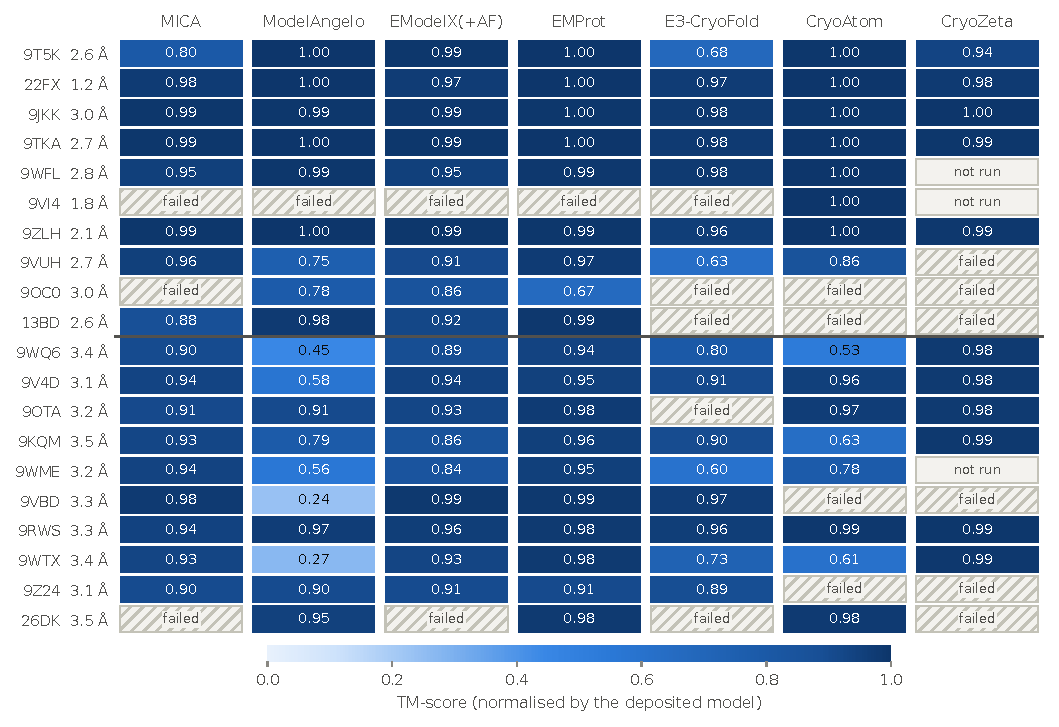
\includegraphics[width=0.93\textwidth]{figures/fig1_tm_score_per_entry.pdf}
\caption{TM-score of every method on every entry (the primary measure, normalised by the deposited model). Entries are ordered by stratum, then by the seeded order of the selection; hatched cells are failed runs. The line separates the two resolution strata.}
\label{fig:heat}
\end{figure}

\subsection{Paired comparison with MICA}\label{sec:paired}
Table~\ref{tab:paired} and Figure~\ref{fig:paired} compare each method with MICA on the entries where both built a model (difference = method minus MICA).
\begin{itemize}
\item \textbf{EMProt} has a higher TM-score than MICA on \HigherTmEmprot{} of \NPairsTmEmprot{} entries; the mean difference is \DiffTmEmprot{} (95\,\% CI \DiffLoTmEmprot{} to \DiffHiTmEmprot{}), the median difference \MedDiffTmEmprot{}, the Wilcoxon $p$ is \PwTmEmprot{} (Holm \PwHolmTmEmprot{}; paired $t$-test, Holm: \PtHolmTmEmprot{}). The difference is small and consistent: it is positive in both strata (\DiffTmEmprotLow{} up to 3.0~\AA{}, \DiffTmEmprotHigh{} above) and EMProt is higher on \HigherTmEmprotHigh{} of the \NPairsTmEmprotHigh{} entries above 3.0~\AA{}.
\item \textbf{EModelX(+AF)} is not different from MICA: mean difference \DiffTmEmodelx{} (\DiffLoTmEmodelx{} to \DiffHiTmEmodelx{}), higher on \HigherTmEmodelx{} and lower on \LowerTmEmodelx{} of \NPairsTmEmodelx{} entries, Wilcoxon Holm $p$ = \PwHolmTmEmodelx{}.
\item \textbf{E3-CryoFold} is lower than MICA: \DiffTmEthree{} (\DiffLoTmEthree{} to \DiffHiTmEthree{}) over \NPairsTmEthree{} entries, lower on \LowerTmEthree{} of them; Wilcoxon Holm $p$ = \PwHolmTmEthree{}, but the $t$-test with Holm correction gives \PtHolmTmEthree{}.
\item \textbf{ModelAngelo} has a mean difference of \DiffTmAngelo{} (\DiffLoTmAngelo{} to \DiffHiTmAngelo{}) but a median difference of \MedDiffTmAngelo{} (higher on \HigherTmAngelo{}, lower on \LowerTmAngelo{} of \NPairsTmAngelo{} entries); the Wilcoxon Holm $p$ is \PwHolmTmAngelo{} and the $t$-test Holm $p$ is \PtHolmTmAngelo{}. The mean is carried by the entries above 3.0~\AA{}: up to 3.0~\AA{} the mean difference is \DiffTmAngeloLow{} (\DiffLoTmAngeloLow{} to \DiffHiTmAngeloLow{}, $n$ = \NPairsTmAngeloLow{}); above 3.0~\AA{} it is \DiffTmAngeloHigh{} (\DiffLoTmAngeloHigh{} to \DiffHiTmAngeloHigh{}, $n$ = \NPairsTmAngeloHigh{}), with ModelAngelo lower on \LowerTmAngeloHigh{} of them and a Wilcoxon Holm $p$ of \PwHolmTmAngeloHigh{} (\PtHolmTmAngeloHigh{} for the $t$-test).
\item \textbf{CryoAtom} (added after the first version) is not different from MICA over all entries: mean difference \DiffTmCryoatom{} (\DiffLoTmCryoatom{} to \DiffHiTmCryoatom{}), median difference \MedDiffTmCryoatom{}, higher on \HigherTmCryoatom{} and lower on \LowerTmCryoatom{} of \NPairsTmCryoatom{} entries, Wilcoxon Holm $p$ = \PwHolmTmCryoatom{} ($t$-test: \PtHolmTmCryoatom{}). Up to 3.0~\AA{} the mean difference is \DiffTmCryoatomLow{} (\DiffLoTmCryoatomLow{} to \DiffHiTmCryoatomLow{}, $n$ = \NPairsTmCryoatomLow{}); above 3.0~\AA{} it is \DiffTmCryoatomHigh{} (\DiffLoTmCryoatomHigh{} to \DiffHiTmCryoatomHigh{}, $n$ = \NPairsTmCryoatomHigh{}), with CryoAtom lower on \LowerTmCryoatomHigh{} of them; this is not clear after the correction (Wilcoxon Holm $p$ = \PwHolmTmCryoatomHigh{}, $t$-test \PtHolmTmCryoatomHigh{}). The \NPairsTmCryoatom{} pairs leave out six entries: the three without a MICA model (26DK, 9VI4, 9OC0) and the other three on which CryoAtom ran out of GPU memory (13BD, 9VBD, 9Z24).
\item \textbf{CryoZeta} (added after the first version) has a higher TM-score than MICA on \HigherTmCryozeta{} of the \NPairsTmCryozeta{} entries where both built a model and a lower one on \LowerTmCryozeta{}: mean difference \DiffTmCryozeta{} (\DiffLoTmCryozeta{} to \DiffHiTmCryozeta{}), median difference \MedDiffTmCryozeta{}, Wilcoxon Holm $p$ = \PwHolmTmCryozeta{} ($t$-test: \PtHolmTmCryozeta{}). Up to 3.0~\AA{} the mean difference is \DiffTmCryozetaLow{} (\DiffLoTmCryozetaLow{} to \DiffHiTmCryozetaLow{}, $n$ = \NPairsTmCryozetaLow{}); above 3.0~\AA{} it is \DiffTmCryozetaHigh{} (\DiffLoTmCryozetaHigh{} to \DiffHiTmCryozetaHigh{}, $n$ = \NPairsTmCryozetaHigh{}), with CryoZeta higher on \HigherTmCryozetaHigh{} of them (Wilcoxon Holm $p$ = \PwHolmTmCryozetaHigh{}, $t$-test \PtHolmTmCryozetaHigh{}). The one entry where CryoZeta is lower is 9ZLH, by less than 0.01. Up to 3.0~\AA{} the mean comes from one entry, 9T5K, where MICA reaches 0.80; on the other four the two methods differ by less than 0.01. The pairs are the entries that CryoZeta finished in the free GPU time; the \NFailedCryozeta{} failures and the \NNotRunCryozeta{} entries not run are not in them, so the comparison holds for these entries and not for the twenty.
\end{itemize}
The rank correlation of the TM-score with the resolution is weak for MICA (Spearman $\rho$ = \RhoResTmMica{}, $p$ = \RhoPResTmMica{}) and stronger for ModelAngelo ($\rho$ = \RhoResTmAngelo{}, $p$ = \RhoPResTmAngelo{}), EMProt (\RhoResTmEmprot{}, \RhoPResTmEmprot{}), EModelX(+AF) (\RhoResTmEmodelx{}, \RhoPResTmEmodelx{}) and above all CryoAtom (\RhoResTmCryoatom{}, \RhoPResTmCryoatom{}); the TM-score of CryoZeta, whose lowest value is \TmMinCryozeta{}, shows no relation to it (\RhoResTmCryozeta{}, \RhoPResTmCryozeta{}, $n$ = \RhoNResTmCryozeta{}); the correlations of the TM-score with the number of residues are all weak (Table~\ref{tab:corr}, Appendix).

\begin{table}[t]
\centering\small
\caption{Paired comparison of the TM-score with MICA on the entries where both methods built a model (method minus MICA; 95\,\% bootstrap CI of the mean difference; two-sided Wilcoxon signed-rank test and paired $t$-test, both with Holm correction over the \NFamilyWord{} methods; counts of entries where the method is higher, lower or equal).}
\label{tab:paired}
\fitwidth{\begin{tabular}{lrccrrrc}
\toprule
Method & Pairs & Mean difference [95\% CI] & Median diff. & Wilcoxon $p$ & Holm $p$ & $t$-test Holm $p$ & higher / lower / equal \\
\midrule
\multicolumn{8}{l}{\emph{All entries}} \\
ModelAngelo & 17 & $-$0.15 [$-$0.28, $-$0.03] & 0.00 & 0.207 & 0.621 & 0.114 & 7 / 10 / 0 \\
EModelX(+AF) & 17 & 0.00 [$-$0.02, 0.03] & 0.00 & 0.818 & 1.000 & 0.827 & 9 / 8 / 0 \\
EMProt & 17 & 0.04 [0.02, 0.06] & 0.02 & $<$0.001 & $<$0.001 & 0.033 & 16 / 1 / 0 \\
E3-CryoFold & 15 & $-$0.08 [$-$0.14, $-$0.03] & $-$0.03 & 0.007 & 0.034 & 0.089 & 2 / 13 / 0 \\
CryoAtom & 14 & $-$0.06 [$-$0.15, 0.02] & 0.00 & 0.761 & 1.000 & 0.392 & 9 / 5 / 0 \\
CryoZeta & 11 & 0.05 [0.02, 0.07] & 0.05 & 0.007 & 0.034 & 0.033 & 10 / 1 / 0 \\
\midrule
\multicolumn{8}{l}{\emph{Resolution $\leq$ 3.0 \AA}} \\
ModelAngelo & 8 & 0.02 [$-$0.06, 0.09] & 0.01 & 0.250 & 0.875 & 1.000 & 6 / 2 / 0 \\
EModelX(+AF) & 8 & 0.02 [$-$0.01, 0.08] & 0.00 & 1.000 & 1.000 & 1.000 & 3 / 5 / 0 \\
EMProt & 8 & 0.05 [0.01, 0.10] & 0.02 & 0.016 & 0.094 & 0.532 & 7 / 1 / 0 \\
E3-CryoFold & 7 & $-$0.07 [$-$0.16, $-$0.00] & $-$0.01 & 0.109 & 0.547 & 0.944 & 1 / 6 / 0 \\
CryoAtom & 7 & 0.03 [$-$0.03, 0.09] & 0.00 & 0.219 & 0.875 & 1.000 & 6 / 1 / 0 \\
CryoZeta & 5 & 0.03 [$-$0.00, 0.08] & 0.00 & 0.438 & 0.875 & 1.000 & 4 / 1 / 0 \\
\midrule
\multicolumn{8}{l}{\emph{Resolution $>$ 3.0 to 4.0 \AA}} \\
ModelAngelo & 9 & $-$0.30 [$-$0.48, $-$0.13] & $-$0.36 & 0.020 & 0.098 & 0.055 & 1 / 8 / 0 \\
EModelX(+AF) & 9 & $-$0.01 [$-$0.04, 0.01] & 0.00 & 1.000 & 1.000 & 0.317 & 6 / 3 / 0 \\
EMProt & 9 & 0.03 [0.02, 0.04] & 0.03 & 0.004 & 0.023 & 0.014 & 9 / 0 / 0 \\
E3-CryoFold & 8 & $-$0.09 [$-$0.17, $-$0.02] & $-$0.03 & 0.039 & 0.125 & 0.252 & 1 / 7 / 0 \\
CryoAtom & 7 & $-$0.15 [$-$0.27, $-$0.01] & $-$0.16 & 0.219 & 0.438 & 0.252 & 3 / 4 / 0 \\
CryoZeta & 6 & 0.06 [0.05, 0.07] & 0.06 & 0.031 & 0.125 & $<$0.001 & 6 / 0 / 0 \\
\bottomrule
\end{tabular}
}
\end{table}

\begin{figure}[t]
\centering
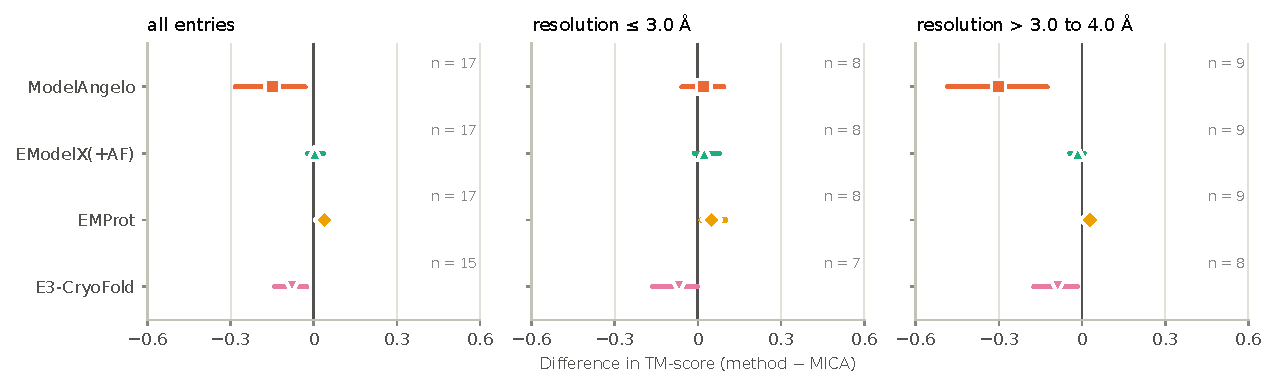
\includegraphics[width=\textwidth]{figures/fig2_paired_differences.pdf}
\caption{Difference in TM-score between each method and MICA (mean and 95\,\% bootstrap CI), for all entries and for each resolution stratum; positive values favour the other method.}
\label{fig:paired}
\end{figure}

\subsection{What the other measures say}\label{sec:othermeasures}
The ranking by TM-score is not an artefact of fragmentation or of extra copies. ModelAngelo writes its models as several chains; US-align's multi-chain mode counts one fragment per deposited chain, so its TM-score mixes accuracy and continuity. With the fragment-agnostic TM-score (Table~\ref{tab:fns}) the difference between ModelAngelo and MICA shrinks to \DiffFnsAngelo{} (\DiffLoFnsAngelo{} to \DiffHiFnsAngelo{}; Wilcoxon Holm $p$ = \PwHolmFnsAngelo{}), EModelX(+AF) stays equal (\DiffFnsEmodelx{}), EMProt stays higher (\DiffFnsEmprot{}, Holm $p$ = \PwHolmFnsEmprot{}) and E3-CryoFold lower (\DiffFnsEthree{}, Holm $p$ = \PwHolmFnsEthree{}); CryoAtom is not different from MICA on this score (\DiffFnsCryoatom{}, \DiffLoFnsCryoatom{} to \DiffHiFnsCryoatom{}; Holm $p$ = \PwHolmFnsCryoatom{}) and CryoZeta stays higher (\DiffFnsCryozeta{}, \DiffLoFnsCryozeta{} to \DiffHiFnsCryozeta{}; Holm $p$ = \PwHolmFnsCryozeta{}). The C$\alpha$ match (precision) is lowest for EMProt (median \CamMedEmprot{} against \CamMedMica{} for MICA) because EMProt builds \CovMedEmprot{} times the deposited number of residues (median; up to \CovMaxEmprot{} times), that is, every copy it finds in the map; the same holds for ModelAngelo in a few entries (coverage up to \CovMaxAngelo{}) and for CryoAtom (median C$\alpha$ match \CamMedCryoatom{}, coverage up to \CovMaxCryoatom{}, that is, many more residues than the deposit); CryoZeta also builds more residues than the deposit (median coverage \CovMedCryozeta{}, up to \CovMaxCryozeta{}; median C$\alpha$ match \CamMedCryozeta{}). MICA builds about the deposited number of residues (median coverage \CovMedMica{}) because its input is one AF3 prediction per unique chain; only in 13BD did it build clearly more than the deposit (coverage \CovMaxMica{}; the next highest is \CovSecondMica{}). The C$\alpha$ quality score, which does not punish extra copies, gives \CaqMedMica{} for MICA, \CaqMedAngelo{} for ModelAngelo, \CaqMedEmodelx{} for EModelX(+AF), \CaqMedEmprot{} for EMProt \CaqMedEthree{} for E3-CryoFold, \CaqMedCryoatom{} for CryoAtom and \CaqMedCryozeta{} for CryoZeta (medians, \%). The median sequence match of MICA is \SqmMedMica{}\,\%, and its median RMSD over the aligned residues is \RmsdMedMica{}~\AA{} for \AliMedMica{} aligned residues, against \RmsdMedAngelo{}~\AA{} for \AliMedAngelo{} for ModelAngelo, whose models align over fewer residues, so RMSDs are not comparable across methods (all measures: Table~\ref{tab:allmetrics}, Figure~\ref{fig:dist}).

\subsection{Failures scored as zero}
If a failed run counts as zero on every measure (Table~\ref{tab:zero}), the mean TM-score over all \NEntries{} entries is \ZeroMeanMica{} for MICA (95\,\% CI \ZeroLoMica{}--\ZeroHiMica{}), \ZeroMeanAngelo{} for ModelAngelo, \ZeroMeanEmodelx{} for EModelX(+AF), \ZeroMeanEmprot{} for EMProt, \ZeroMeanEthree{} for E3-CryoFold and \ZeroMeanCryoatom{} for CryoAtom. For CryoZeta the mean is taken over the \ZeroNCryozeta{} entries on which it ran, its \NFailedCryozeta{} failures counted as zero (the entries not run are not failures and are left out): \ZeroMeanCryozeta{} (95\,\% CI \ZeroLoCryozeta{}--\ZeroHiCryozeta{}); the second variant of Table~\ref{tab:zero} counts the entries not run as zero as well. On this footing neither ModelAngelo, EModelX(+AF), CryoAtom nor CryoZeta differs from MICA: the mean differences are \ZeroDiffAngelo{}, \ZeroDiffEmodelx{}, \ZeroDiffCryoatom{} and \ZeroDiffCryozeta{} (Holm $p$ = \ZeroPwHolmAngelo{}, \ZeroPwHolmEmodelx{}, \ZeroPwHolmCryoatom{} and \ZeroPwHolmCryozeta{}). For CryoZeta the difference is taken over the \ZeroNCryozeta{} entries on which it ran, with the results of MICA on the same entries; it is negative because CryoZeta failed on 9Z24, 13BD, 9VBD and 9VUH, where MICA built a model. The failures of CryoAtom and CryoZeta are limits of the 15~GB GPU, of the RAM and of the run limit and not errors of the programs, as those of MICA are limits of the free machine. EMProt remains higher (\ZeroDiffEmprot{}; Holm $p$ \ZeroPwHolmEmprot{}) and E3-CryoFold lower (\ZeroDiffEthree{}; Holm $p$ = \ZeroPwHolmEthree{}). If the \NRerunMica{} reruns counted as failures as well, MICA would have \FirstModels{} models with a mean TM-score of \FirstTmMean{}, and a mean of \FirstZeroMean{} over all 20 entries.

\subsection{Docking and its effect on MICA}\label{sec:dockresults}
MICA's own docking could not be run on a free machine (Section~\ref{sec:mica}), so the placements of the AF3 domains in the map are coarse and unverified. Pass~3 docked \DockDockedThree{} of \DockDomainsThree{} domains (Table~\ref{tab:docking}); \DockModeFull{} entries are fully docked, \DockModePartial{} partly and \DockModeNone{} not at all.

\paragraph{Docked against no docked input.}
On the \DockEffectN{} entries that ran with and without docked input (all fully docked), the TM-score is \DockEffectMeanDocked{} with and \DockEffectMeanNoDock{} without docked input; the mean difference is \DockEffectMean{} (95\,\% CI \DockEffectLo{} to \DockEffectHi{}), Wilcoxon $p$ = \DockEffectP{}, higher with docked input on \DockEffectHigher{} and lower on \DockEffectLower{} entries (Table~\ref{tab:dockeffect}). The differences are small (the largest are 9KQM and 9VUH), but they go in the expected direction, which is weak evidence that the coarse placements carry information. Without docked input MICA still uses the AF3 structures when it builds the chains, so this is not a comparison with MICA without AlphaFold.

\paragraph{By docking mode.}
The \ModeFullModels{} models of fully docked entries have a mean TM-score of \ModeFullTmMean{} (range \ModeFullTmMin{}--\ModeFullTmMax{}), the \ModePartialModels{} models of partly docked entries \ModePartialTmMean{} (\ModePartialTmMin{}--\ModePartialTmMax{}); the three lowest TM-scores of MICA are those of \ModeLowThreeList{}, and \ModeLowThreePartial{} of these entries are partly docked. This is a description and not a test, because the entries also differ in size and resolution, but it points to the same side: where the free-compute docking left a domain unplaced, MICA was less accurate, so the docking deviation more probably understates than overstates MICA. The initial C$\alpha$ model that MICA's network writes before the chains are built from the AF3 structures has a median TM-score of \MicaVarInitTmMed{}, against \MicaVarAllTmMed{} for the final model (Table~\ref{tab:variants}); a large part of MICA's accuracy on these maps comes from the step that uses the AF3 structures (the AF3 predictions themselves were not scored).

\subsection{Novelty and run time}
Only \NIdentLow{} entries have a chain at 30\,\% identity or less to any pre-2026 PDB chain (9TKA, 9VBD, 26DK), and MICA failed on one of them, so the planned low-identity analysis has \NPairsTmEmprotNovel{} pairs and is not tested; the TM-scores on these entries are in Table~\ref{tab:perentry}. Over all entries the TM-score of MICA is not related to the identity to older entries (Spearman $\rho$ = \RhoIdentTmMica{}, $p$ = \RhoPIdentTmMica{}), and no method shows a relation with $p$ below 0.05 (smallest $p$ of the \NMethodsWord{} methods: \RhoIdentMinP{}; Table~\ref{tab:corr}).

Run times are only indicative (Table~\ref{tab:runtime}, Figure~\ref{fig:runtime}). The median time of MICA is \RtMedMica{} min per entry (range \RtMinMica{} to \RtMaxMica{}; \RtTotMica{}~h in total for programs 1 to 3 including docking), against \RtMedAngelo{} min for ModelAngelo, \RtMedEmodelx{} for EModelX(+AF), \RtMedEmprot{} for EMProt, \RtMedEthree{} for E3-CryoFold and \RtMedCryoatom{} for CryoAtom (range \RtMinCryoatom{} to \RtMaxCryoatom{}) and \RtMedCryozeta{} for CryoZeta (range \RtMinCryozeta{} to \RtMaxCryozeta{}, failed runs included; the time of CryoZeta includes the search for the alignments on the ColabFold server). The baselines were timed while a second program used the other GPU, MICA's program~3 ran one entry at a time, and most of MICA's time on a large map goes into model building on one CPU core. The whole benchmark, including every failed attempt and the first two docking passes, used \GpuSessionHours{}~h of GPU sessions and \CpuSessionHours{}~h of CPU sessions (\NSessions{} sessions, Table~\ref{tab:sessions}).
